\documentclass[12pt]{article}
\usepackage{a4}
\usepackage[english]{babel}
\setlength{\parindent}{0.35cm}
\pagestyle{headings}
\usepackage{graphicx}
%Multiple picture in one figure
\usepackage{subfig}
\usepackage{listings}
\usepackage{color}
%Zum Zeilen umbrechen in Tabellen
\usepackage{pbox}
\usepackage{wrapfig}
%Floating-Umgebungen
\usepackage{float}
%Math-Environment
\usepackage{amsmath}
%Better SI-Units
\usepackage{siunitx}
\DeclareSIUnit\century{century}
\DeclareSIUnit\year{yr}
%Using Appendix
\usepackage[title]{appendix}
%Using URL
\usepackage[hidelinks]{hyperref}
%Using Colored Tables
\usepackage{colortbl}
%Using text-based symbols
\usepackage{textcomp}
\usepackage{gensymb}

% New/Renewing Commands
\newcommand{\eV}{\electronvolt}
\newcommand{\keV}{\kilo\electronvolt}
\newcommand{\meV}{\mega\electronvolt}
\newcommand{\gray}{\rowcolor[gray]{.90}}

%Configure geometry
\usepackage{geometry}
\geometry{
	a4paper,
	left=3cm,
	right=3cm,
	top=3cm,
	bottom = 3cm,
	}

\lstset{
	language=C++,
	basicstyle=\small\ttfamily,
	keywordstyle=\color{blue}\ttfamily,
	stringstyle=\color{red}\ttfamily,
	commentstyle=\color{green}\ttfamily,
	morecomment=[l][\color{magenta}]{\#},
}


\begin{document}
	
\title{
	\textbf{\huge{Irradiation of SiPMs}}}
\author{by \\ Lukas Nies \\ Justus-Liebig-Universit\"at Gie\ss{}en \\ II. Physikalisches Institut}
\date{June and July 2017 
}
\maketitle

\section{Methodology}

To grant temperature stability, the SiPMs and the Raspberry Pi are placed in a climate chamber, the temperature is set to $T=\SI{25}{\degreeCelsius}$ for all precision measurements. \par 
This setup is shown in figure \ref{fig1}: The climate chamber by WEISS? contains two aluminum boxes with the SiPM, a temperature sensor, the ''HV" distribution board and a paper box with a Raspberry Pi 2. The HV board \cite{HV_board}, which is currently under development for the EMC barrel of the PANDA experiment at FAIR (GSI), has been chosen to perform the IV-scanning because of availability and easy programmability. The board is controlled by a Raspberry Pi 2 and too reads out a temperature sensor which is directly connected to the SiPM. To avoid parasitic light and surface leakage, the SiPM is cleaned with ethanol and wrapped in black tape. A Keithley Sourcemeter powers the HV board, a PC controls the Raspberry via Ethernet. The temperature settings can be set by a terminal. \par 
\begin{figure}[b]
	\centering
	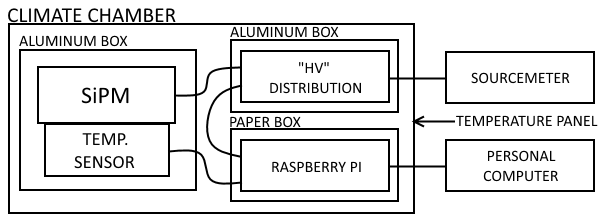
\includegraphics[width=0.85\linewidth]{./graphics/scheme_precision.png}
	\caption{Mesurement setup in Giessen.}
	\label{fig1}
\end{figure} 
The IV-curves are scanned from $I=\SI{0}{\nano\ampere}$ to $I\approx\SI{1000}{\nano\ampere}$ and back to $I=\SI{0}{\nano\ampere}$. This is looped five times. The step range is given by the digital potentiometer (10bit) at the HV board, a small hysteresis for the current is know (see \cite{HV_board}). For each potentiometer position (voltage), the current is measured 100 times and is then averaged. This results in ten IV-curves per SiPM which should improve precision.     


\section{Measurements}
blank
\subsection{Before irradiation}
blank
\begin{figure}[H]
	\subfloat[SiPM \#1] {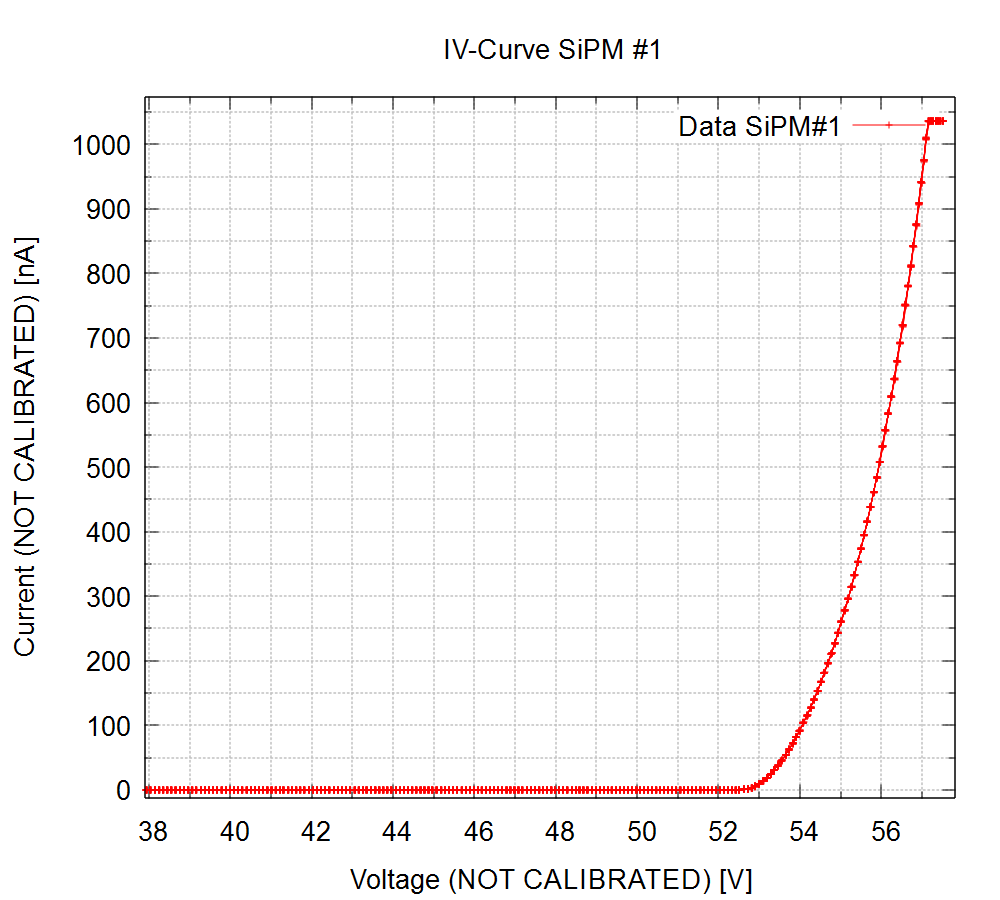
\includegraphics[width=0.49\textwidth]{../before/plots/sipm_1.png}}
	\hfill
	\subfloat[SiPM \#1 (log)] {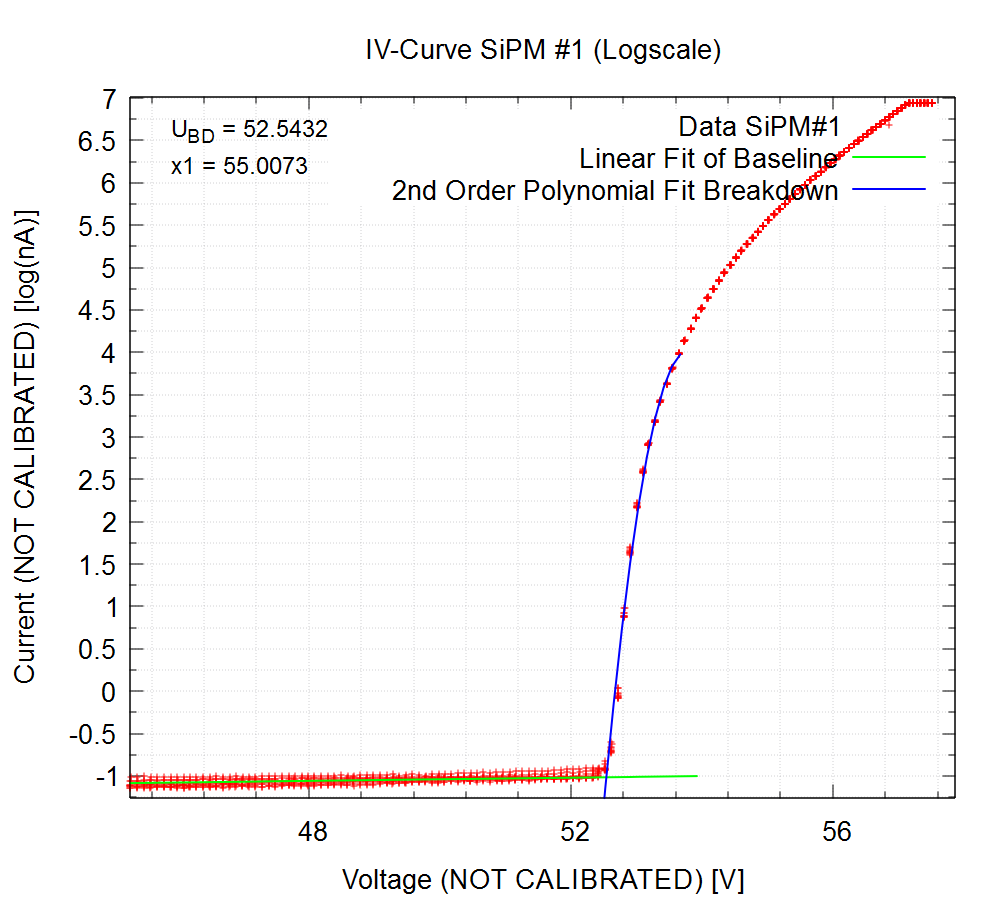
\includegraphics[width=0.49\textwidth]{../before/plots/sipm_1_log.png}}
	\hfill
	\subfloat[SiPM \#2] {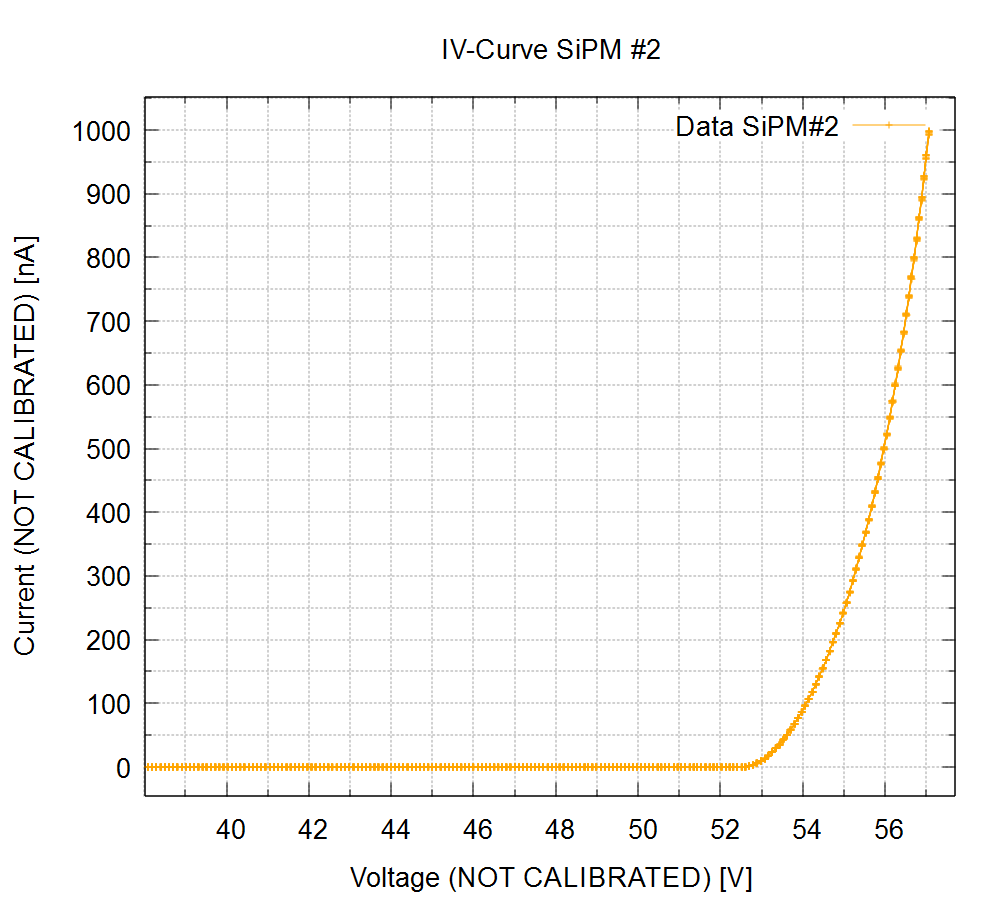
\includegraphics[width=0.49\textwidth]{../before/plots/sipm_2.png}}
	\hfill
	\subfloat[SiPM \#2 (log)] {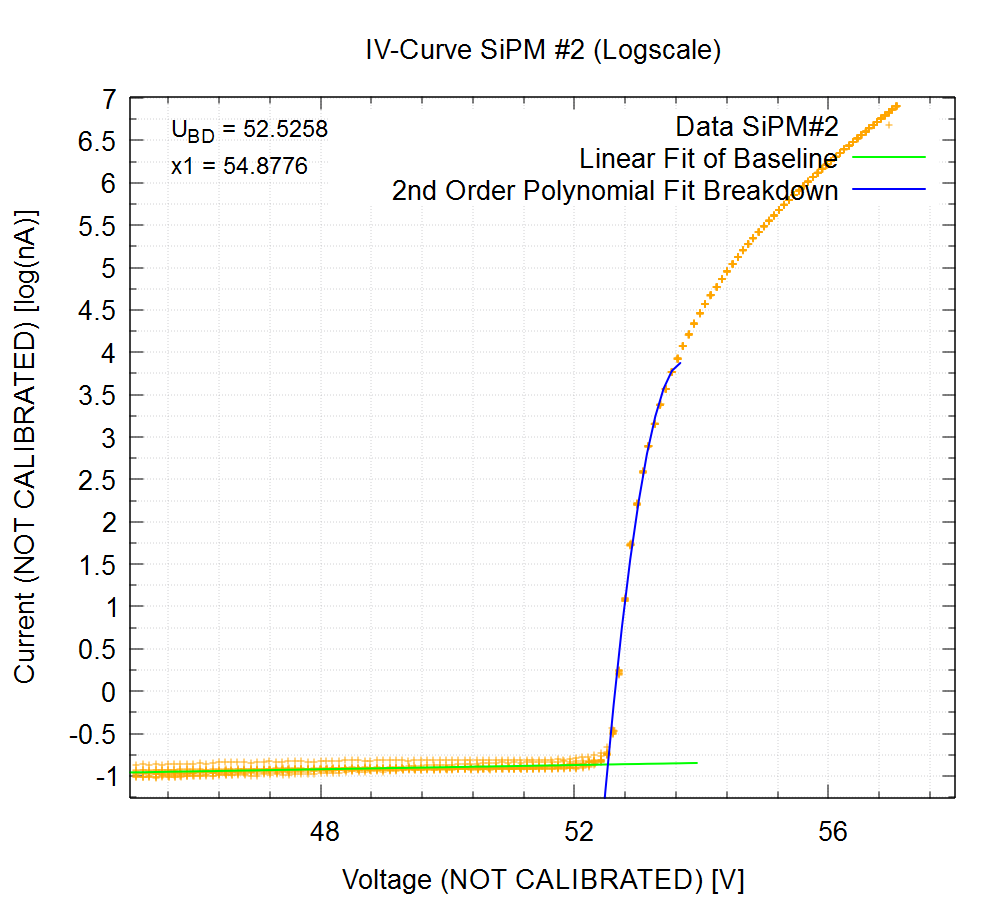
\includegraphics[width=0.49\textwidth]{../before/plots/sipm_2_log.png}}
	\hfill
	\subfloat[SiPM \#3] {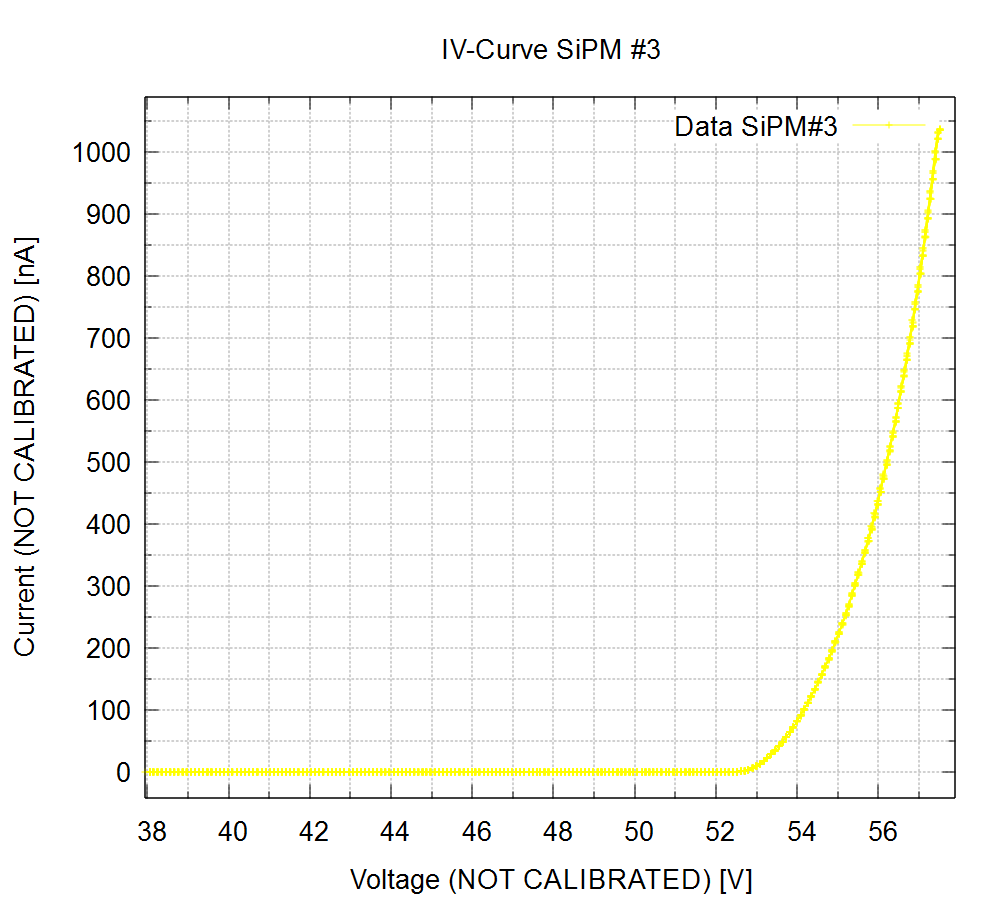
\includegraphics[width=0.49\textwidth]{../before/plots/sipm_3.png}}
	\hfill
	\subfloat[SiPM \#3 (log)] {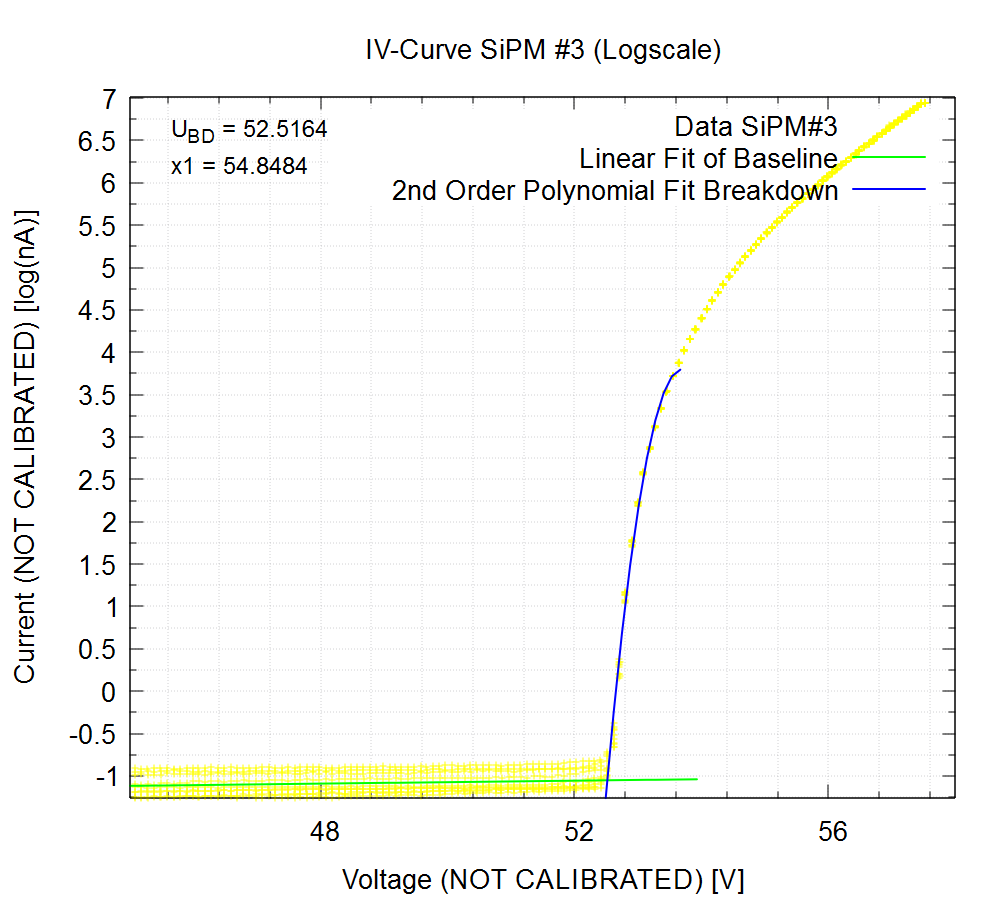
\includegraphics[width=0.49\textwidth]{../before/plots/sipm_3_log.png}}
	\hfill
	\caption[]{Comparison of different SiPMs.}
\end{figure}
\begin{figure}[H]
	\subfloat[SiPM \#4] {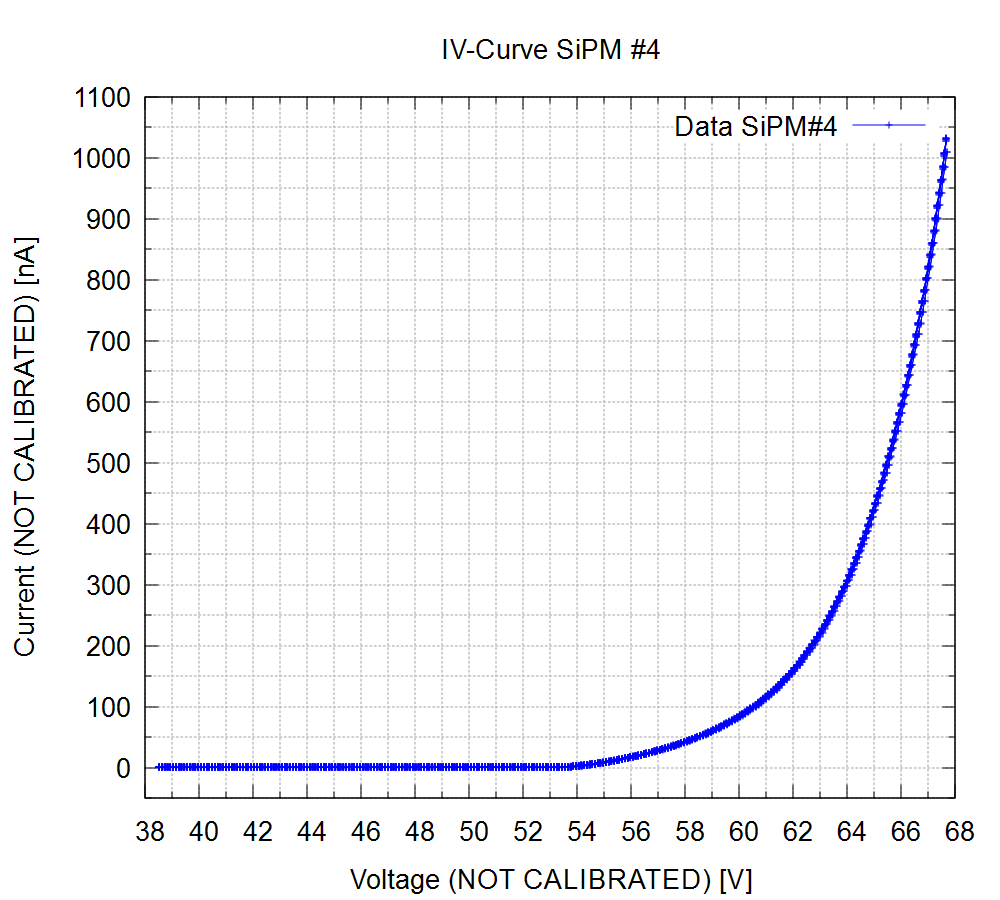
\includegraphics[width=0.49\textwidth]{../before/plots/sipm_4.png}}
	\hfill
	\subfloat[SiPM \#4 (log)] {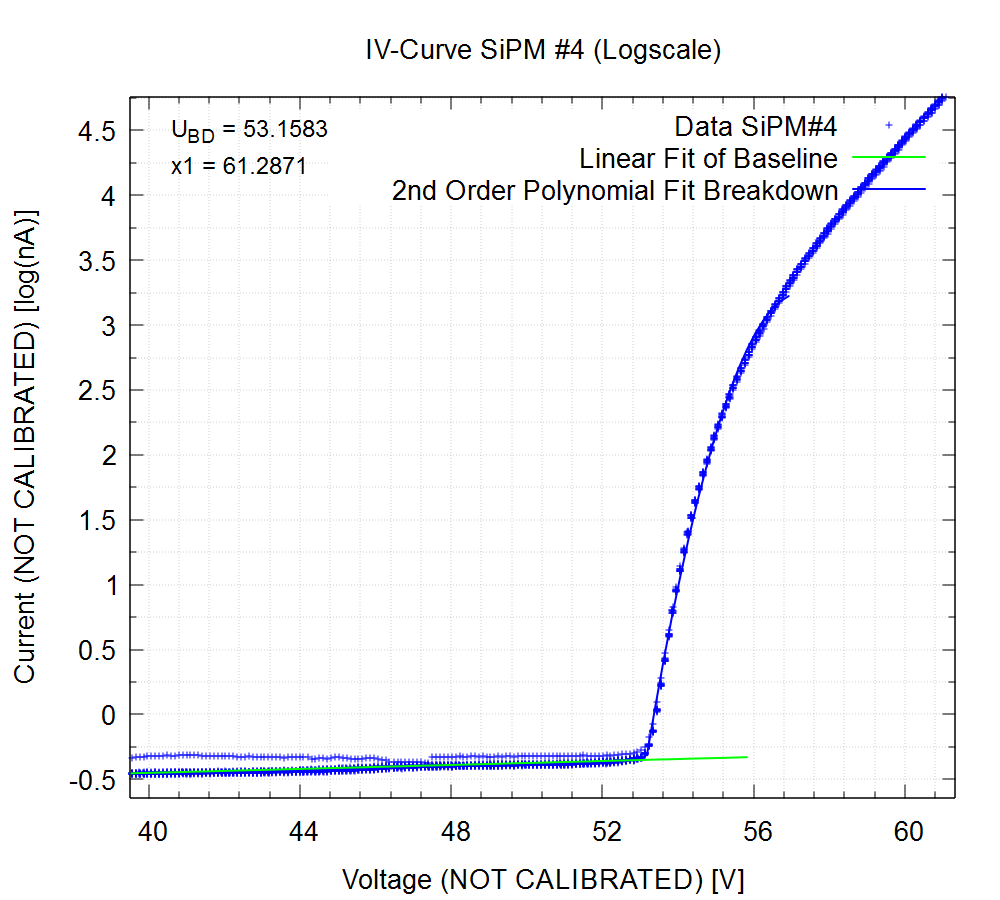
\includegraphics[width=0.49\textwidth]{../before/plots/sipm_4_log.png}}
	\hfill
	\subfloat[SiPM \#5] {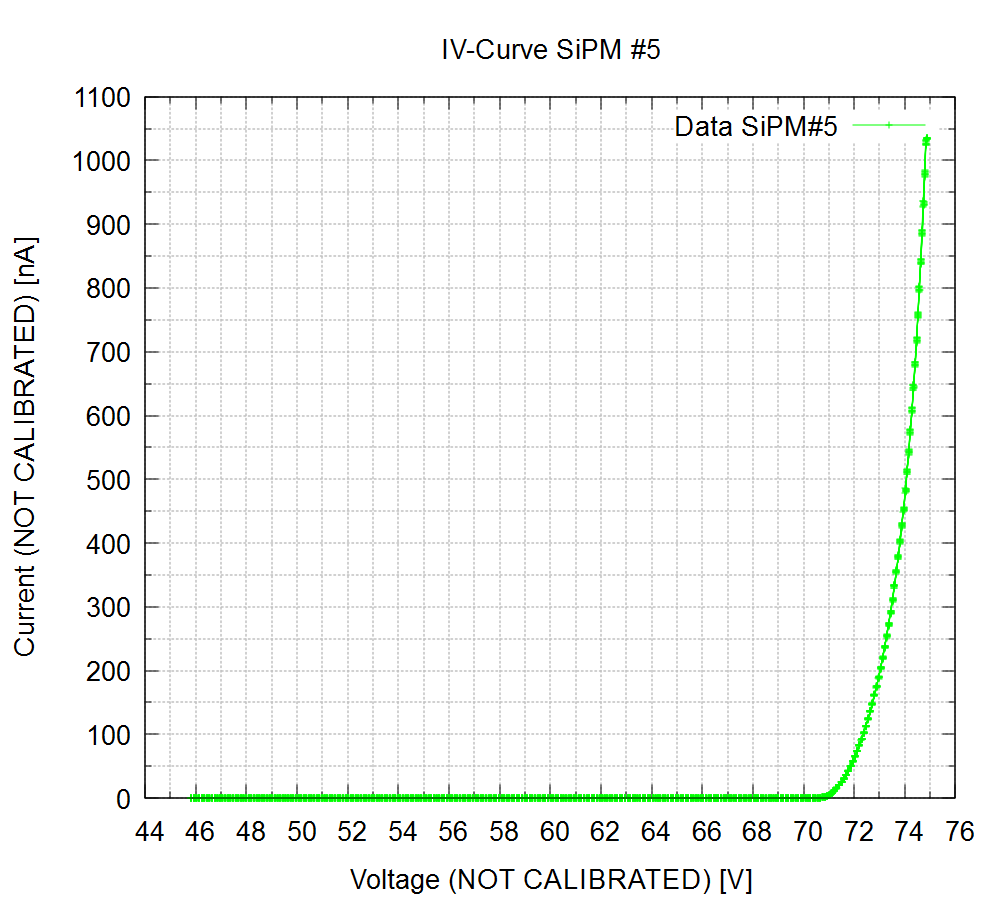
\includegraphics[width=0.49\textwidth]{../before/plots/sipm_5.png}}
	\hfill
	\subfloat[SiPM \#5 (log)] {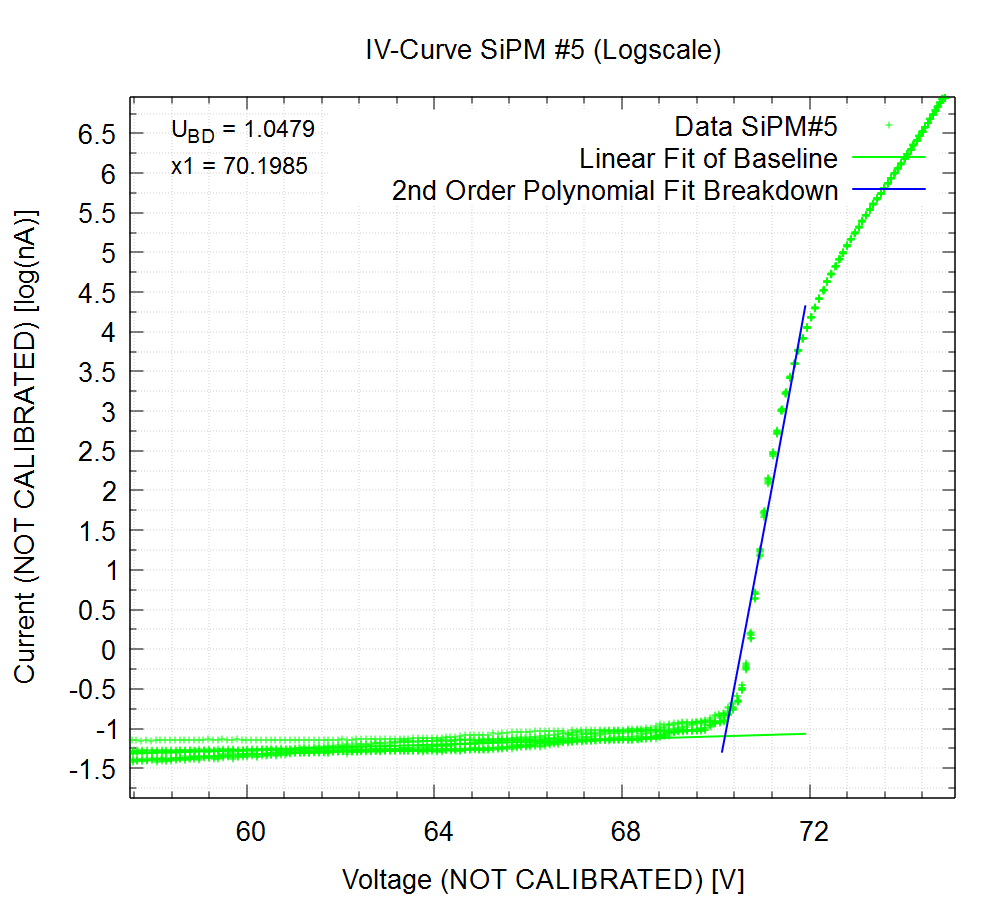
\includegraphics[width=0.49\textwidth]{../before/plots/sipm_5_log.png}}
	\hfill
	\subfloat[SiPM \#6] {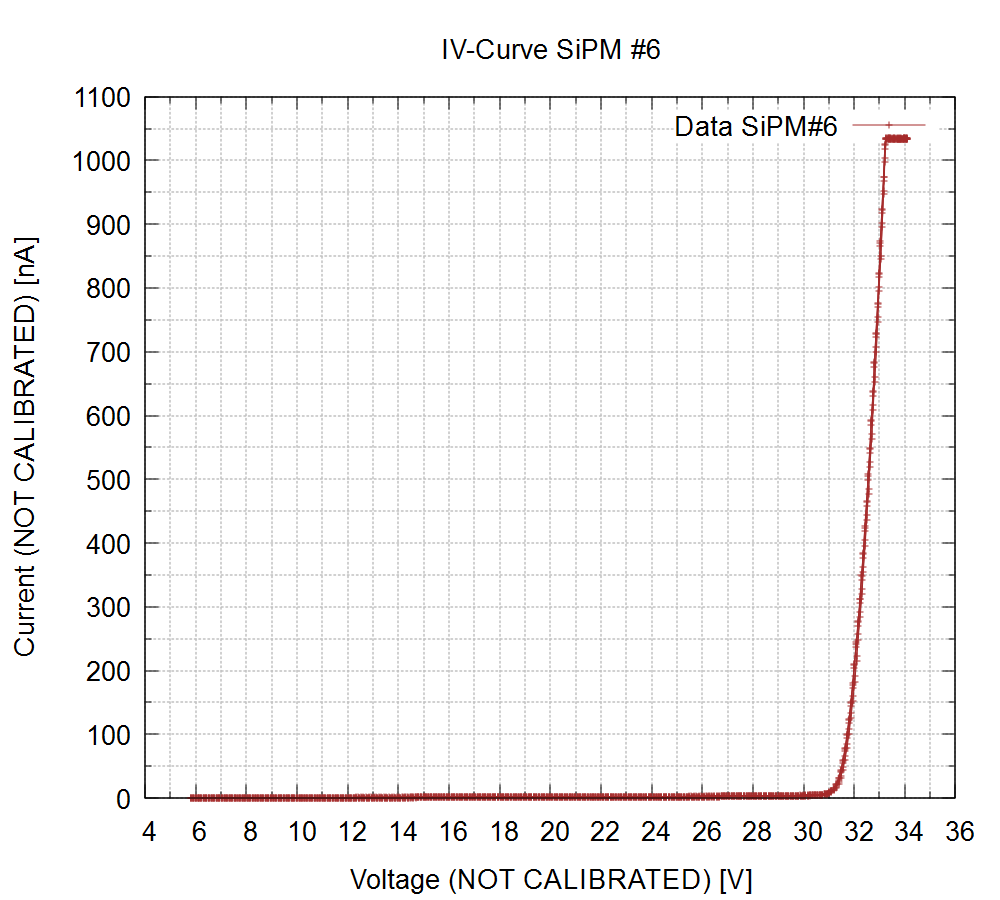
\includegraphics[width=0.49\textwidth]{../before/plots/sipm_6.png}}
	\hfill
	\subfloat[SiPM \#6 (log)] {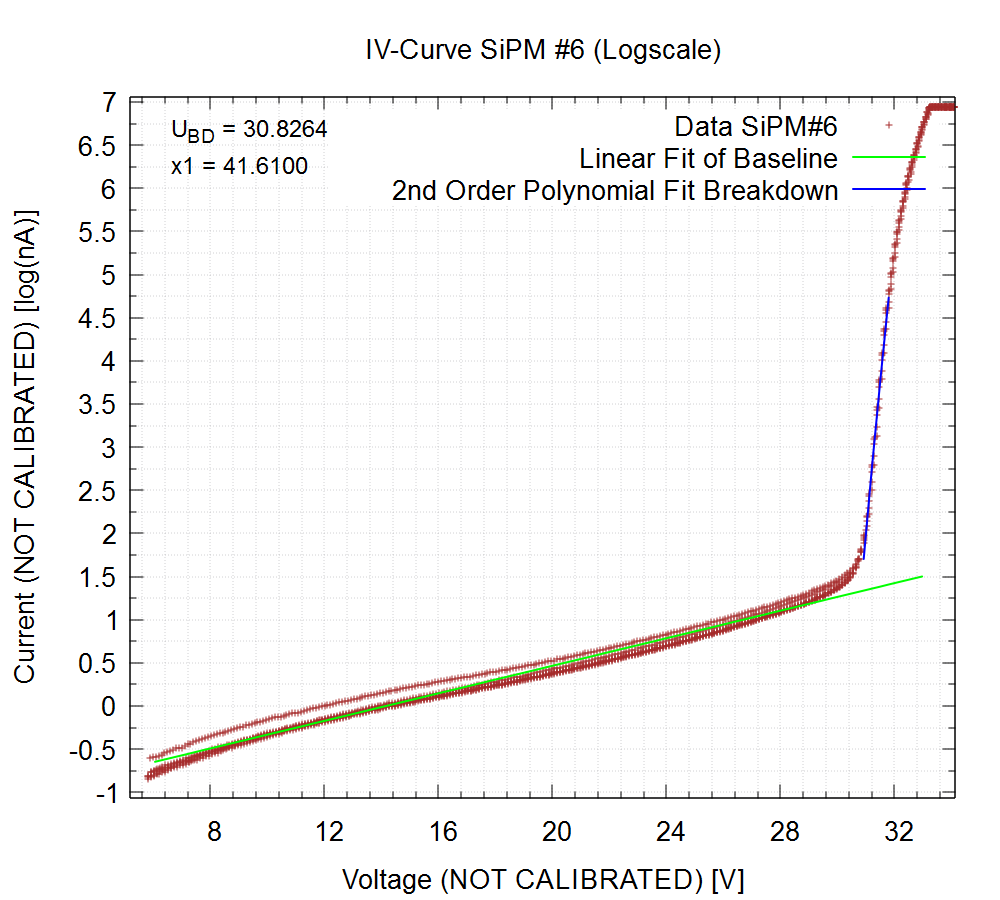
\includegraphics[width=0.49\textwidth]{../before/plots/sipm_6_log.png}}
	\hfill
	\caption[]{Comparison of different SiPMs part 2.}
\end{figure}
\begin{figure}[H]
	\subfloat[SiPM \#4] {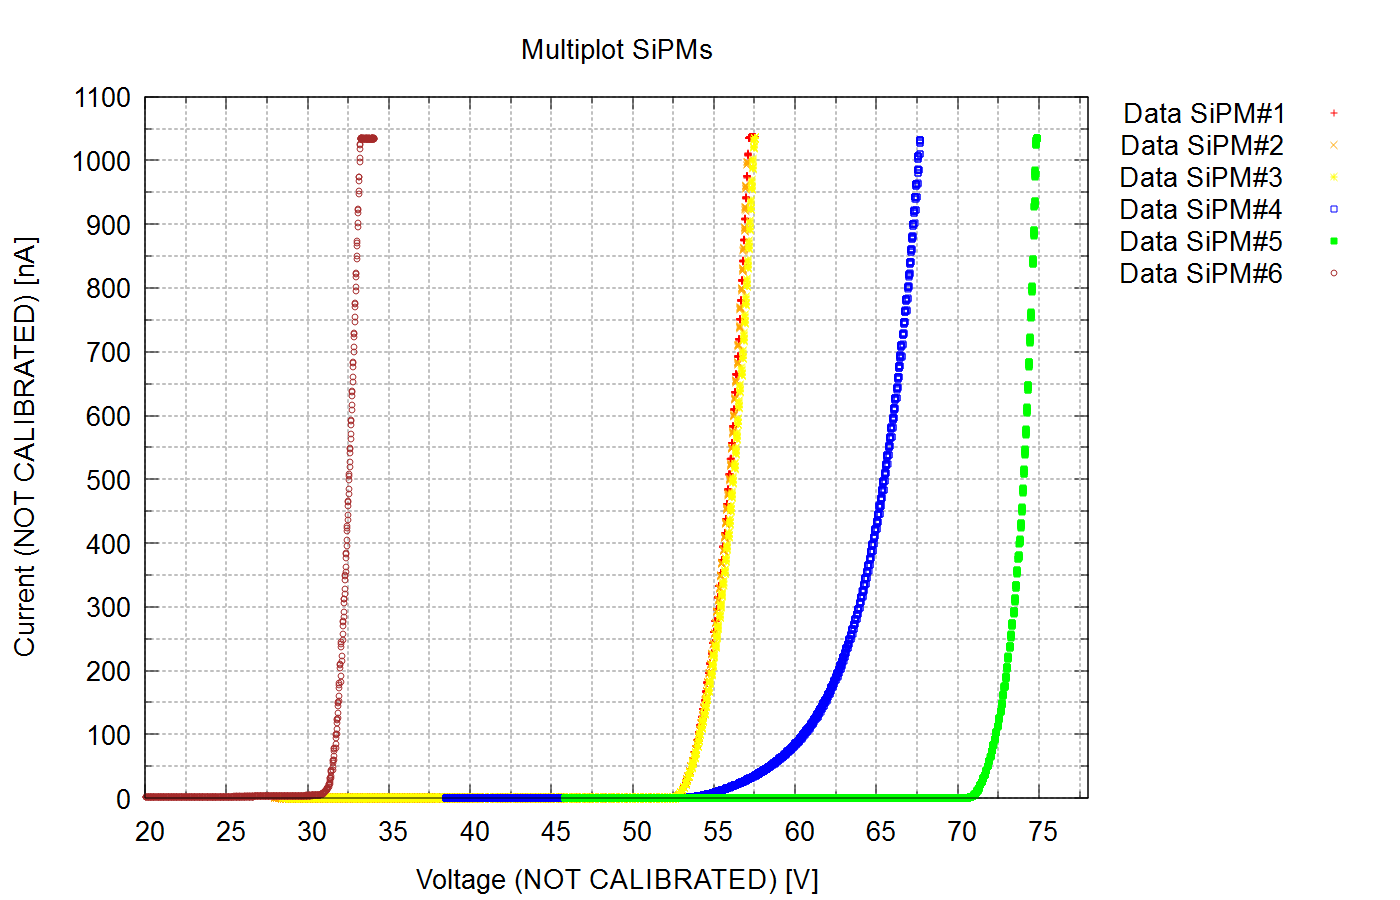
\includegraphics[width=1\textwidth]{../before/plots/multiplot.png}}
	\hfill
	\subfloat[SiPM \#4 (log)] {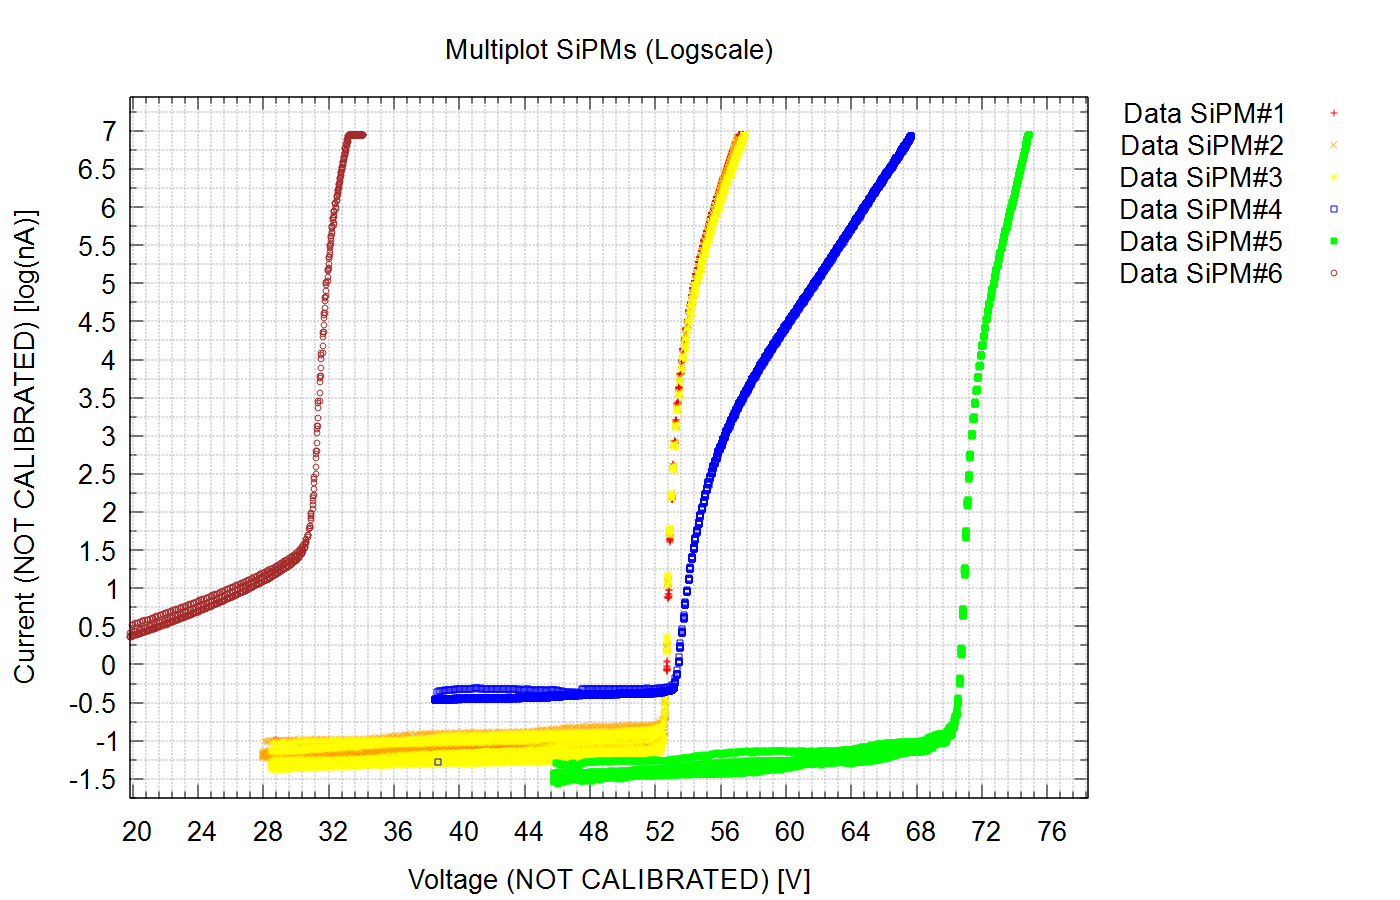
\includegraphics[width=1\textwidth]{../before/plots/multiplot_log.png}}
	\hfill
	\caption[]{Comparison of different SiPMs part 3.}
\end{figure}


\bibliographystyle{unsrt}
\bibliography{./bib}


	
	
	
	
	
	
	
	
	
	
	
	
	
	
	
\end{document}